\chapter{Introduction}\label{chap:Intro}%\addcontentsline{toc}{chapter}{\nameref{chap:Intro}}
%\markboth{INTRODUCTION}{}
\mylocaltoc

\section{Revue bibliographique}

\begin{itemize}
    \item Théorie linéaire de Rott : \cite{rott_damped_1969, rott_thermally_1973, rott_thermally_1975, rott_thermally_1976, zouzoulas_thermally_1976, rott_thermoacoustics_1980, muller_thermally_1983} 
    \item $f_\nu$ et $f_\kappa$ : \cite{swift_thermoacoustics_2017,di_giulio_wire_2023}
    \item Tortuosité et matériaux poreux : \cite{johnson_theory_1987, drummond_laminar_1984}
    \item Phase optimale : \cite{poignand_etude_2006}
    \item Thermocouples dans noyau TA : \cite{duffourd_refrigerateur_2001, penelet_etude_2004}
    \item Bilan de chaleur dans coeur TA : \cite{penelet_etude_2004}
    \item Mélange de gaz : \cite{belcher_working_1999}
    \item Géométrie coaxiale : \cite{poignand_analysis_2013, poignand_thermoacoustic_2011, tijani_study_2008, ramadan_design_2021}
    \item Géométrie compacte : \cite{poignand_etude_2006}
    \item Convection naturelle : \cite{ross_influence_2003, hireche_numerical_2019, pan_visualization_2012, bianchi_transferts_2004, babaei_investigation_2010, gardner_cascade_2003}
    \item Convection naturelle dans les poreux : \cite{shiina_critical_2010, kvernvold_nonlinear_1979, richard_critere_1981, horton_convection_1945}
    \item Streaming : \cite{so_internal_2006, bailliet_acoustic_2001, ramadan_experimental_2018}
    \item Analogies électroac en TA : \cite{wakeland_use_2000, backhaus_thermoacoustic-stirling_2000, poignand_analysis_2013}
    \item Electroac générale : \cite{rossi_electroacoustique_1986, novak_measurement_2019}
    \item Pertes latérales : \cite{penelet_etude_2004, guedra_etudes_2012}
    \item Non uniformité de température sur la section : \cite{penelet_etude_2004}
    \item Conduction dans les stack et meshgrids : \cite{hsu_effective_1996, li_effective_2006, g_correlations_2022}
\end{itemize}

\section{Contexte du travail}

\section{Bases de thermoacoustique}
\subsection{Concepts généraux}
Les machines thermoacoustique utilisent les interactions visqueuses et thermiques entre un gaz et un matériau solide poreux ou d’un empilement de plaques (\textit{stack} en anglais) placé dedans lors d’un cycle de compression-détente de ce gaz. En particulier, les pression, volume et température, qui sont liées par les lois thermodynamiques, sont des grandeurs d’intérêt en thermoacoustique dont la théorie linéaire est en grande partie écrite par Rott et Swift au cours des années 1980 \cite{rott_damped_1969, rott_thermally_1973, rott_thermally_1975, rott_thermally_1976, zouzoulas_thermally_1976, rott_thermoacoustics_1980, muller_thermally_1983}

Deux schémas de principe des machines thermoacoustiques sont présentés figure~\ref{fig:MoteurVSFrigoTA}. Le mode moteur (figure~\ref{fig:MoteurTA}) transforme l’énergie thermique en énergie acoustique, tandis que le mode pompe à chaleur et réfrigérateur (figure~\ref{fig:FrigoTA}) génère un flux de chaleur sous l'action d'une énergie acoustique. 

Dans un moteur thermoacoustique, le chauffage d'un côté du matériau poreux apporte de l'énergie à une parcelle de gaz située à proximité de ce côté du stack. Son volume augmente alors et pousse les autres parcelles de gaz attenantes à l'intérieur du stack, en direction de l'autre extrémité plus froide. Elle cèdent de l'énergie au solide, leur volume diminue et elle retrouvent leur position initiale, où le cycle recommence. Finalement, c'est un travail acoustique qui est généré.

La pompe à chaleur fonctionne en suivant le cycle thermodynamique inverse : l'onde acoustique fournit un travail au fluide et le compresse, ce qui fait augmenter sa température. À l'extrémité du matériau poreux dont la température initiale est inférieure à celle du fluide, une certaine quantité de chaleur est extraite du fluide. La parcelle de fluide se déplace alors dans le matériau poreux, se détend et refroidit, puis extrait à son tour une quantité de chaleur au solide. Au final, un flux de chaleur de la source à refroidir vers l'ambiant est provoqué de proche en proche.\smallskip

\begin{figure}[!ht]
	\centering
	\begin{subfigure}{.47\textwidth}
		\centering
		\external{fig_MoteurTA}
%        \externalremake
		\begin{tikzpicture}
    \draw[white] (0,-3) -- ++(0,6);

	\draw[MatlabOrange](-3,2.5) -- ++(6,0) node[near end,below]{$T_c$};
	\draw[MatlabBlue](-3,-2.5) -- ++(6,0) node[near end,above]{$T_f$};
			
	\fill[gray!50, rounded corners](-1.5,-1) rectangle (1.5,1) node[midway]{\textcolor{black}{Moteur}};
			
	\draw[<-,very thick,MatlabBlue](0,-2.4) -- (0,-1.1) node[midway,left]{$Q_f$};
	\draw[<-,very thick,MatlabOrange](0,1.1) -- (0,2.4) node[midway,left]{$Q_c$};
	\draw[->,very thick](1.6,0) -- ++(2.4-1.1,0) node[midway,above]{$W_{ac}$};
\end{tikzpicture}
		\caption{moteur}
		\label{fig:MoteurTA}
	\end{subfigure}
	\hfill% \vline \hfill
	\begin{subfigure}{.47\textwidth}
		\centering
		\external{fig_FrigoTA}
%        \externalremake
		\begin{tikzpicture}
    \draw[rounded corners,dashed,very thick,draw=black,fill=black!5!white] (-3.5,-3) rectangle ++(7,6.5) node[below left]{Objet de cette thèse};

	\draw[MatlabOrange](-3,2.5) -- ++(6,0) node[near end,below]{$T_c$};
	\draw[MatlabBlue](-3,-2.5) -- ++(6,0) node[near end,above]{$T_f$};
	
	\fill[gray!50,rounded corners](-1.5,-1) rectangle (1.5,1) node[midway,align=center]{\textcolor{black}{\shortstack{Pompe\\à chaleur}}};
			
	\draw[->,very thick,MatlabBlue](0,-2.4) -- (0,-1.1) node[midway,left]{$Q_f$};
	\draw[->,very thick,MatlabOrange](0,1.1) -- (0,2.4) node[midway,left]{$Q_c$};
	\draw[->,very thick](-1.6-2.4+1.1,0) -- ++(2.4-1.1,0) node[midway,above]{$W_{ac}$};
\end{tikzpicture}
		\caption{pompe à chaleur}
		\label{fig:FrigoTA}
	\end{subfigure}
	\caption[Schémas de principe d'un moteur et d'une pompe à chaleur thermoacoustique]{Schémas de principe d'un moteur et d'une pompe à chaleur thermoacoustique. D'après \cite{swift_thermoacoustics_2017}.}
	\label{fig:MoteurVSFrigoTA}
\end{figure}

Après avoir succintement défini le mode de fonctionnement d'une machine, il est nécessaire de présenter de type de propagation d'onde prenant place au sein de son noyau. Il existe deux comportements asymptotiques qui dépendent de la forme du résonateur de la machine : les ondes stationnaires d'une part et les ondes progressives d'autre part. Ces deux cas sont radicalement différents, car le déphasage entre la pression acoustique $p$ et la vitesse acoustique $v$ est de \ang{90} dans le premier cas, et \ang{0} dans le second.

%\begin{figure}[!ht]
%    \centering
%    \begin{subfigure}{\textwidth}
%    	\centering
%    	\external{fig_OndesStatio}
%%    	\externalremake
%    	\begin{tikzpicture}
    \def\height{5cm};
    \def\width{.45\textwidth};
    \def\spx{1.1cm};
    \def\spy{.5cm};
    \def\legx{.5cm};
    \def\legy{.25cm};
    \def\Vamp{.6};
    
    \begin{axis}[name=pv,height=\height,width=\width,
    domain=0:3.14,xmin=0,xmax=3.14,no markers,
    xtick={0,{3.14/2},3.14},xticklabels={$0$,$\frac{L}{2}$,$L$},
    ytick={0,\Vamp,1},yticklabels={$0$,$+\tilde V$,$+\tilde P$},legend entries={$\tilde p$,$\tilde v$},
    at={(-\width,0)},anchor=south west,
    ylabel near ticks, yticklabel pos=right,
    legend pos=south west
    ]
    \addplot[PythonBlue,line width=3pt] {cos(deg(x))}; 
    \addplot[dashed,PythonOrange,line width=3pt] {\Vamp*sin(deg(x))};
    \end{axis}
    
    \draw (pv.north west) -- ($(pv.west)+(-2*\legx,0)$) -- (pv.south west) -- cycle;
    \fill[black!40] ($(pv.west)+(-2.01*\legx,-.5*\height/3)$) rectangle ++(\legx,\height/3);  
\end{tikzpicture}
%    	\caption{}
%    	\label{fig:OndesStatio}
%    \end{subfigure}
%%\end{figure}
%%\\[10pt]
%%\begin{figure}[!ht]
%	\begin{subfigure}{\textwidth}
%    	\centering
%	    \external{fig_OndesProg}
%%	    \externalremake
%	    \begin{tikzpicture}
    \def\allong{1};
    \def\height{5cm};
    \def\width{.3\textwidth};
    
    \begin{axis}[name=pv,height=\height,width=\width,
    domain=0:7,xmin=0,xmax=7,no markers,
    xtick={0,{3.14/2},3.14},xticklabels=\empty,
    ytick={-1,-.7,0,.7,1},yticklabels={$-\tilde P$,$-\tilde V$,$0$,$+\tilde V$,$+\tilde P$},
    hide axis,
    legend entries={$\tilde p$,$\tilde v$},
    legend pos=south west
    ]
    \addplot[smooth,PythonBlue,line width=3pt] {cos(deg(.5*x+18))}; 
    \addplot[smooth,dashed,PythonOrange,line width=3pt] {.7*cos(deg(.5*x+18))};
    \end{axis}
    
    
    \draw[dashed, very thick] (pv.north west) -- ($(pv.north west)+(\allong,0)$);
    \draw[very thick] ($(pv.north west)+(\allong,0)$) -- ($(pv.north east)+(-\allong,0)$);
    \draw[dashed, very thick] ($(pv.north east)+(-\allong,0)$) -- (pv.north east);
    
    \draw[dashed, very thick] (pv.south west) -- ($(pv.south west)+(\allong,0)$);
    \draw[very thick] ($(pv.south west)+(\allong,0)$) -- ($(pv.south east)+(-\allong,0)$);
    \draw[dashed, very thick] ($(pv.south east)+(-\allong,0)$) -- (pv.south east);
    
    
\end{tikzpicture}
%	    \caption{}
%	    \label{fig:OndesProg}
%    \end{subfigure}
%    \caption{\subref{fig:OndesStatio} ondes stationnaires et \subref{fig:OndesProg} ondes progressives dans un guide d'ondes.}
%    \label{fig:Ondes}
%\end{figure}

Les cycles thermodynamiques évoqués plus tôt sont différents en fonction de chaque cas : un volume élémentaire de gaz dans un stack de machine à ondes stationnaires est soumis à un cycle de Brayton, tandis que dans un régénérateur de machine à ondes progressives le volume suit un cycle de Stirling. Ces cycles sont présentés respectivement dans les figures \ref{fig:CycleBrayton} et \ref{fig:CycleStirling}.

\begin{figure}[!htp]
	\centering
	\begin{subfigure}{.47\textwidth}
		\centering
		\external{fig_1_BraytonDepComp}
%        \externalremake
		\begin{tikzpicture}[scale=.8]
	\fill[left color=PythonRed,right color=PythonBlue](-3,-2) rectangle (3,-3) node[midway,text=white]{Plaque};
	\draw[dotted,thick] (-2,-3.2) -- (-2,1.2) node[above,right]{$-\xi_{0}$};
	\draw[dotted,thick] (2,-3.2) -- (2,1.2) node[above,right]{$+\xi_{0}$};
		
	\draw(2,0) circle (1);
	\draw[dashed](-2,0) circle (.5);
			
	\draw[<->,PythonGreen] (0,-1.9) -- (0,0) node[above,right]{$\delta_{\kappa,\nu}$};
\end{tikzpicture}
		\caption{déplacement et compression adiabatique}
		\label{fig:CycleBrayton_DepCompAdiab}
	\end{subfigure}
	%
	\begin{subfigure}{.47\textwidth}
		\centering
		\external{fig_2_BraytonQfluidePlaque}
%        \externalremake
		\begin{tikzpicture}[scale=.8,>=latex]
	\fill[left color=PythonRed,right color=PythonBlue](-3,-2) rectangle (3,-3) node[midway,text=white]{Plaque};
	\draw[dotted,thick] (-2,-3.2) -- (-2,1.2) node[above,right]{$-\xi_{0}$};
	\draw[dotted,thick] (2,-3.2) -- (2,1.2) node[above,right]{$+\xi_{0}$};		
		
	\draw(-2,0) circle (.5);
			
	\draw[PythonRed,->,very thick](-2,-.6) -- (-2,-1.9) node[midway,right]{$\deriv q$};
			
	\draw[<->,PythonGreen] (0,-1.9) -- (0,0) node[above,right]{$\delta_{\kappa,\nu}$};
\end{tikzpicture}
		\caption{cession de chaleur du fluide à la plaque}
		\label{fig:CycleBrayton_QFluidePlaque}
	\end{subfigure}
	
	\vspace{5mm}
	%
	\begin{subfigure}{.47\textwidth}
		\centering
		\external{fig_3_BraytonDepDet}
%        \externalremake
		\begin{tikzpicture}[scale=.8]
	\fill[left color=PythonRed,right color=PythonBlue](-3,-2) rectangle (3,-3) node[midway,text=white]{Plaque};
	\draw[dotted,thick] (-2,-3.2) -- (-2,1.2) node[above,right]{$-\xi_{0}$};
	\draw[dotted,thick] (2,-3.2) -- (2,1.2) node[above,right]{$+\xi_{0}$};
					
	\draw(-2,0) circle (.5);
	\draw[dashed](2,0) circle (1);
			
	\draw[<->,PythonGreen] (0,-1.9) -- (0,0) node[above,right]{$\delta_{\kappa,\nu}$};
\end{tikzpicture}
		\caption{déplacement et détente adiabatique}
		\label{fig:CycleBrayton_DepDetAdiab}
	\end{subfigure}
	%
	\begin{subfigure}{.47\textwidth}
		\centering
		\external{fig_4_BraytonQPlaqueFluide}
%        \externalremake
		\begin{tikzpicture}[scale=.8]
	\fill[left color=PythonRed,right color=PythonBlue](-3,-2) rectangle (3,-3) node[midway,text=white]{Plaque};
	\draw[dotted,thick] (-2,-3.2) -- (-2,1.2) node[above,right]{$-\xi_{0}$};
	\draw[dotted,thick] (2,-3.2) -- (2,1.2) node[above,right]{$+\xi_{0}$};
			
	\draw(2,0) circle (1);
			
	\draw[PythonBlue,->,very thick](2,-1.9) -- (2,-1.1) node[midway,right]{$\deriv q$};
			
	\draw[<->,PythonGreen] (0,-1.9) -- (0,0) node[above,right]{$\delta_{\kappa,\nu}$};
\end{tikzpicture}
		\caption{cession de chaleur de la plaque au fluide}
		\label{fig:CycleBrayton_QPlaqueToFluide}
	\end{subfigure}	
	\caption[Cycle de Brayton des machines à ondes stationnaires]{Cycle thermodynamique de Brayton en fonctionnement réfrigérateur/pompe à chaleur à ondes stationnaires. Les traits pleins dénotent l'état initial de l'étape, les traits pointillés, l'état final.}
	\label{fig:CycleBrayton}
\end{figure} % Brayton

\begin{figure}[!htp]
	\centering
	\begin{subfigure}{.47\textwidth}
		\centering
		\external{fig_1_StirlingComp}
%        \externalremake
		\begin{tikzpicture}[scale=.8]

	\fill[left color=white, right color=PythonGreen!25!white] (-3,-2) rectangle (-2,1); 
	\fill[PythonGreen!25!white] (-2,1) rectangle (2,-2); 
	\fill[left color=PythonGreen!25!white, right color=white] (2,1) rectangle (3,-2); 
	\shade[upper left=white,upper right=white,
         lower left=white,lower right=PythonGreen!25!white] (-3,1) rectangle (-2,3.5);
	\fill[top color=white, bottom color=PythonGreen!25!white] (-2,3.5) rectangle (2,1);
	\shade[upper left=white,upper right=white,
         lower left=PythonGreen!25!white,lower right=white] (2,1) rectangle (3,3.5);
	

	\fill[left color=PythonRed,right color=PythonBlue](-3,-2) rectangle (3,-3) node[midway,text=white]{Plaque};				
	\draw[dotted,thick] (-2,-3.2) -- (-2,1.2) node[above,right]{$-\xi_1$};
	\draw[dotted,thick] (2,-3.2) -- (2,1.2) node[above,right]{$+\xi_1$};	
		
	\draw(-2,0) circle (1);
	\draw[dashed](-2,0) circle (.5);
			
	\draw[dashed,->,very thick,MatlabOrange](-2,-.6) -- (-2,-1.9) node[midway,right]{$\deriv q$};
			
	\draw[<-,dashed,PythonGreen](0,2.4) node[below,right]{$\delta_{\kappa,\nu}$} -- (0,1.5) ;
	\draw[->,PythonGreen](0,1.5) -- (0,-1.9);
\end{tikzpicture}
		\caption{compression isotherme}
		\label{fig:CycleStirling_Comp}
	\end{subfigure}
	%
	\begin{subfigure}{.47\textwidth}
		\centering
		\external{fig_2_StirlingDep1}
%        \externalremake
		\begin{tikzpicture}[scale=.8]

	\fill[left color=white, right color=PythonGreen!25!white] (-3,-2) rectangle (-2,1); 
	\fill[PythonGreen!25!white] (-2,1) rectangle (2,-2); 
	\fill[left color=PythonGreen!25!white, right color=white] (2,1) rectangle (3,-2); 
	\shade[upper left=white,upper right=white,
         lower left=white,lower right=PythonGreen!25!white] (-3,1) rectangle (-2,3.5);
	\fill[top color=white, bottom color=PythonGreen!25!white] (-2,3.5) rectangle (2,1);
	\shade[upper left=white,upper right=white,
         lower left=PythonGreen!25!white,lower right=white] (2,1) rectangle (3,3.5);

	\fill[left color=PythonRed,right color=PythonBlue](-3,-2) rectangle (3,-3) node[midway,text=white]{Plaque};
	\draw[dotted,thick] (-2,-3.2) -- (-2,1.2) node[above,right]{$-\xi_1$};
	\draw[dotted,thick] (2,-3.2) -- (2,1.2) node[above,right]{$+\xi_1$};
		
	\draw(-2,0) circle (.5);
	\draw[dashed](2,0) circle (.5);
			
	\draw[<-,dashed,PythonGreen](0,2.4) node[below,right]{$\delta_{\kappa,\nu}$} -- (0,1.5) ;
	\draw[->,PythonGreen](0,1.5) -- (0,-1.9);
\end{tikzpicture}
		\caption{déplacement isochore (aller)}
		\label{fig:CycleStirling_DepIsoch1}
	\end{subfigure}
	
	\vspace{5mm}
	%
	\begin{subfigure}{.47\textwidth}
		\centering
		\external{fig_3_StirlingDet}
%        \externalremake
		\begin{tikzpicture}[scale=.8]
	\fill[left color=PythonRed,right color=PythonBlue](-3,-2) rectangle (3,-3) node[midway,text=white]{Plaque};	
	\draw[dotted,thick] (-2,-3.2) -- (-2,1.2) node[above,right]{$-\xi_{0}$};
	\draw[dotted,thick] (2,-3.2) -- (2,1.2) node[above,right]{$+\xi_{0}$};
			
	\draw(2,0) circle (.5);
	\draw[dashed](2,0) circle (1);
			
	\draw[dashed,->,very thick,MatlabBlue](2,-1.9) -- (2,-1.1) node[midway,right]{$\deriv q$};

	\draw[<-,dashed,PythonGreen](0,2.5) node[right]{$\delta_{\kappa,\nu}$} -- (0,1.5) ;
	\draw[->,PythonGreen](0,1.5) -- (0,-1.9);
\end{tikzpicture}
		\caption{détente isotherme}
		\label{fig:CycleStirling_Detente}
	\end{subfigure}
	%
	\begin{subfigure}{.47\textwidth}
		\centering
		\external{fig_4_StirlingDep2}
%        \externalremake
		\begin{tikzpicture}[scale=.8]

	\fill[left color=white, right color=PythonGreen!25!white] (-3,-2) rectangle (-2,1); 
	\fill[PythonGreen!25!white] (-2,1) rectangle (2,-2); 
	\fill[left color=PythonGreen!25!white, right color=white] (2,1) rectangle (3,-2); 
	\shade[upper left=white,upper right=white,
         lower left=white,lower right=PythonGreen!25!white] (-3,1) rectangle (-2,3.5);
	\fill[top color=white, bottom color=PythonGreen!25!white] (-2,3.5) rectangle (2,1);
	\shade[upper left=white,upper right=white,
         lower left=PythonGreen!25!white,lower right=white] (2,1) rectangle (3,3.5);
         
	\fill[left color=PythonRed,right color=PythonBlue](-3,-2) rectangle (3,-3) node[midway,text=white]{Plaque};
	\draw[dotted,thick] (-2,-3.2) -- (-2,1.2) node[above,right]{$-\xi_1$};
	\draw[dotted,thick] (2,-3.2) -- (2,1.2) node[above,right]{$+\xi_1$};
		
	\draw(2,0) circle (1);
	\draw[dashed](-2,0) circle (1);
			
	\draw[<-,dashed,PythonGreen](0,2.4) node[below,right]{$\delta_{\kappa,\nu}$} -- (0,1.5) ;
	\draw[->,PythonGreen](0,1.5) -- (0,-1.9);
\end{tikzpicture}
		\caption{déplacement isochore (retour)}
		\label{fig:CycleStirling_DepIsoch2}
	\end{subfigure}	
	\caption[Cycle de Stirling des machines à ondes progressives]{Cycle thermodynamique de Stirling en fonctionnement réfrigérateur/pompe à chaleur à ondes progressives. Les traits pleins dénotent l'état initial de l'étape, les traits pointillés, l'état final.}
	\label{fig:CycleStirling}
\end{figure} % Stirling



Aux abords d'une paroi se trouvent les couches limites thermiques et visqueuses, dans lesquelles les échanges d'énergie ont lieu. Elles sont respectivement définies par

\begin{subequations}
	\begin{align}
		\delta_{\kappa} &= \sqrt{\frac{2 k}{\rho C_p \omega}} = \sqrt{\frac{2 \kappa}{\omega}}	\label{eq:CouchesLimites_Thermique}\\
		\intertext{et}
		\delta_{\nu} &= \sqrt{\frac{2 \mu}{\rho \omega}} = \sqrt{\frac{2 \nu}{\omega}},	\label{eq:CouchesLimites_Visqueuse}
	\end{align}
	\label{eq:CouchesLimites}%
\end{subequations}
avec $k$ (ou $\kappa$) la conductivité (ou diffusivité) thermique du fluide, $C_p$ sa capacité calorifique à pression constante, $\mu$ (ou $\nu$) sa viscosité dynamique (ou cinématique), $\rho$ sa masse volumique et $\omega = 2\pi f$ la pulsation à laquelle le fluide oscille.

En outre, ces deux épaisseurs de couche limites sont également liées par le nombre de Prandtl $\mathrm{Pr}$, défini par

\begin{subequations}
	\begin{align}
		\Prandtl &= \left(\frac{\delta_{\nu}}{\delta_{\kappa}}\right)^2 \text{, ou} \label{eq:Prandtl_delta}\\
				&= \frac{\mu C_{p}}{k} = \frac{\nu}{\kappa}, \label{eq:Prandtl_MuK_NuKappa}
	\end{align}
	\label{eq:Prandtl}%
\end{subequations}
et qui décrit le rapport de force entre les effets visqueux et thermiques. Dans le cas des machines thermoacoustiques, le nombre de Prandtl doit être le plus faible possible, afin de favoriser les échanges de chaleurs sans perdre d'énergie à cause de la viscosité du fluide. Pour ce faire, il est possible de mélanger des gaz pour abaisser sa valeur \cite{belcher_working_1999} puisque dans le cas des gaz monoatomiques, le nombre de Prandtl ne dépend pas de la température et $\Prandtl=\nicefrac{2}{3}$.

Ces effets visco-thermiques ajoutent des termes dans les équations de l'acoustique, et sont présentés dans les parties qui suivent.

\subsection{\'Equations fondamentales de l'acoustique en fluides dissipatifs}

Un volume de fluide obéit aux lois de conservations de masse, d'énergies et d'état, qui s'écrivent respectivement suivant le système d'équations

\begin{subequations}
	\begin{align}
		\partial_t \rho + \nabla \cdot (\rho \mathbf v) &= 0, \label{eq:ConservMass}\\
		\rho \deriv_t \mathbf v &= -\nabla p + \mu\left( \nabla^2 \mathbf v +\left(\frac13+\frac{\mu_v}{\mu} \right)\nabla\left(\nabla \cdot \mathbf v\right)\right), \label{eq:NavierStokes_QteMvt_base}\\
		\rho T\deriv_t s &= \nabla\cdot (k \nabla T) + \overline{\overline{\sigma}}\cdot \textcolor{red}{\nabla \mathbf v}. \label{eq:ConservEnergie}
	\end{align}
\end{subequations}
en utilisant les variables d'intérêt suivante : la pression $p$, le débit $u$, la vitesse $v$, la masse volumique $\rho$, la température $T$ et l'entropie $s$. Elles sont écrites selon le formalisme de Rott avec les équations

\begin{subequations}
	\begin{multicols}{2}
	\noindent
		\begin{align}
			p(x,t) &= p_0 + \RE \left[p_1(x) e^{i\omega t}\right],\label{eq:pression_rott}\\
			u(x,t) &= \RE \left[u_1(x) e^{i\omega t}\right],\label{eq:debit_rott}\\
			v(x,t) &= \RE \left[v_1(x) e^{i\omega t}\right],\label{eq:vitesse_rott}
	\end{align}
	\begin{align}
			\rho(x,r,t) &= \rho_0(x) + \RE \left[\rho_1(x,r) e^{i\omega t}\right],\label{eq:massVol_rott}\\
			T(x,r,t) &= T_0(x) + \RE \left[T_1(x,r) e^{i\omega t}\right],\label{eq:temperature_rott}\\
			s(x,r,t) &= s_0(x) + \RE \left[s_1(x,r) e^{i\omega t}\right].\label{eq:entropie_rott}
		\end{align}
		\label{eq:variables_rott}
	\end{multicols}
\end{subequations}
Ici, les indices indiquent l'ordre de grandeur, avec en particulier l'indice \num{0} qui dénote une valeur constante à l'ordre \num{0}, et l'indice \num{1} qui signifie l'oscillation à l'ordre \num{1} de la quantité. Il est supposé que le système opère dans un régime linéaire, ce qui se traduit par
\begin{equation}
	\bullet_1 \ll \bullet_0,
	\label{eq:ConditionLinearite}
\end{equation}
où $\bullet$ représente indifféremment la pression, la masse volumique, etc.

Le flux de chaleur thermoacoustique est donné par Swift \cite{swift_thermoacoustics_2017} par
\begin{equation}
	Q_{TA} = \underbrace{\frac{1}{2} \RE\left[pu^* \left( 1 - \frac{f_\kappa - f_\nu^*}{(1 - \Prandtl)(1 - f_\nu^*)} \right) \right]}_{q_{TA}} + \underbrace{\frac{\rho_0 C_p }{\Phi S \omega } \frac{1}{2} \IM \left[ \frac{f_\kappa + \Prandtl f_\nu^*}{(1-\Prandtl)|1-f_\nu|^2} |u|^2\right]}_{k_{TA}} \deriv_x T
	\label{eq:FluxTA_swift}
\end{equation}

\section{\'Etat de l'art}
\subsection{De la recherche fondamentale...}
L'effet thermoacoustique est un phénomène observé depuis les environs du I\ier{} siècle avant notre ère \echaf{src souffleurs de verre + préparation du riz (cours Guillaume ?) ?} \cite{adeff_measurement_1991}

Depuis les années 1970-1980 durant lesquelles les premières machines modernes ont été mises au point, beaucoup de chemin a été parcouru. Le premier moteur à ondes progressives a été construit par Ceperley en 1979 \cite{ceperley_pistonless_1979}, et la première pompe à chaleur par Hofler lors de son doctorat en 1983 \echaf{src}

\subsection{... à des applications industrielles}
Les machines thermoacoustiques sont intéressantes pour l'industrie \echaf{continuer avec cryocooler pour liquéfaction de gaz + TNO/BlueHeart ?}\cite{swift_thermoacoustics_2002, wollan_development_2002, adeff_measurement_1991, garrett_thermoacoustic_1993}

\section{Outils électroacoustiques pour la thermoacoustique}
%\subsection{Transduction électrodynamique}
%Un transducteur est un système qui convertit une forme d'énergie en une autre. En électroacoustique, les haut-parleurs transforment l'énergie électrique en énergie acoustique, ou inversement pour les microphones. Pour réaliser cette transduction, plusieurs technologies existent : électrodynamique, électrostatique...
%
%\begin{figure}[!ht]
%    \centering
%    \external{fig_HautParleur}
%%    \externalremake
%    \begin{tikzpicture}[scale=.9]
    \def\polelong{6};
    \def\polethick{.5};
    \def\magx{2};
    \def\magy{2};
    \def\depth{3};
    \def\dustcap{\depth/10};
    \def\diam{10};
    \def\VCdiam{1.5*\polethick};
    \def\VClen{3};
    \def\VCwire{.15};
    \def\Nwire{20};
    \def\LineThick{.1};

    %\def\theta{atan(.5*\diam/\depth)};
    
%\draw (0,0) node[]{O};

%%%%%%%%%%%%%% Pole piece
\fill[black!15] (0,0) rectangle ++(-.5*\polelong,\polethick);
\fill[black!15] (-\polethick,\polethick) rectangle ++(\polethick,\magy+\polethick);
\fill[black!15] (-.5*\polelong,\magy+\polethick) rectangle ++(.3*\polelong,\polethick);
    
%%%%%%%%%%%%%% Magnet
\fill[black!30] (-.6*\polelong,\polethick) rectangle ++(\magx,\magy);
    
%%%%%%%%%%%%%% Voice coil
\draw[MatlabBlue] ({-\VCdiam},{1.5*\polethick+\magy-.5*\VClen}) -- ++(0,\VClen) node (VCtop){};
\foreach[parse=true] \y in {1,...,{\Nwire-1}}{
    \draw[MatlabBlue] ({-\VCdiam-.5*\VCwire},{\y*\VClen/\Nwire+1.5*\polethick+\magy-.5*\VClen}) circle (.5*\VCwire);
    }
    
%%%%%%%%%%%%%% Basket
\draw[line width={\LineThick/0.0352777778}] ({-.6*\polelong+\magx},{2*\polethick+\magy+.5*\LineThick}) -| ($(VCtop.center)+(1.5*\polethick-.6*\polelong,0)$) node(Bbot){} -- ++(-.5*\diam,\depth) -- ++(-.5,0) node(Btop){} -- ++(0,.5);
    
%%%%%%%%%%%%%% Suspension and membrane
\draw[MatlabOrange,line width={\LineThick/0.0352777778}] ($(Btop.center)+(.5*\LineThick,\LineThick)$) -- ++(.75,0) arc (180:0:.5) coordinate(susp);
\draw[MatlabYellow,line width={\LineThick/0.0352777778}] (susp) -- (VCtop.center) arc (180:90:{\VCdiam} and {\dustcap});
\draw[MatlabOrange,decorate,decoration=snake,line width={.5*\LineThick/0.0352777778}] (Bbot.center) -- (VCtop.center);
    
    %%%%%%%%%%%%%% Mirror
    \begin{scope}[xscale=-1,yscale=1]
        %\def\theta{atan(.5*\diam/\depth)};
    
%\draw (0,0) node[]{O};

%%%%%%%%%%%%%% Pole piece
\fill[black!15] (0,0) rectangle ++(-.5*\polelong,\polethick);
\fill[black!15] (-\polethick,\polethick) rectangle ++(\polethick,\magy+\polethick);
\fill[black!15] (-.5*\polelong,\magy+\polethick) rectangle ++(.3*\polelong,\polethick);
    
%%%%%%%%%%%%%% Magnet
\fill[black!30] (-.6*\polelong,\polethick) rectangle ++(\magx,\magy);
    
%%%%%%%%%%%%%% Voice coil
\draw[MatlabBlue] ({-\VCdiam},{1.5*\polethick+\magy-.5*\VClen}) -- ++(0,\VClen) node (VCtop){};
\foreach[parse=true] \y in {1,...,{\Nwire-1}}{
    \draw[MatlabBlue] ({-\VCdiam-.5*\VCwire},{\y*\VClen/\Nwire+1.5*\polethick+\magy-.5*\VClen}) circle (.5*\VCwire);
    }
    
%%%%%%%%%%%%%% Basket
\draw[line width={\LineThick/0.0352777778}] ({-.6*\polelong+\magx},{2*\polethick+\magy+.5*\LineThick}) -| ($(VCtop.center)+(1.5*\polethick-.6*\polelong,0)$) node(Bbot){} -- ++(-.5*\diam,\depth) -- ++(-.5,0) node(Btop){} -- ++(0,.5);
    
%%%%%%%%%%%%%% Suspension and membrane
\draw[MatlabOrange,line width={\LineThick/0.0352777778}] ($(Btop.center)+(.5*\LineThick,\LineThick)$) -- ++(.75,0) arc (180:0:.5) coordinate(susp);
\draw[MatlabYellow,line width={\LineThick/0.0352777778}] (susp) -- (VCtop.center) arc (180:90:{\VCdiam} and {\dustcap});
\draw[MatlabOrange,decorate,decoration=snake,line width={.5*\LineThick/0.0352777778}] (Bbot.center) -- (VCtop.center);    
    \end{scope}
    
    %\draw[dash dot,PythonGreen] (0,-\polethick) -- ++(0,{3*\polethick+\magy+\VClen+\depth});
    
    \draw[->,MatlabOrange] (-1.5*\polelong,{4*\polethick+\magy+1}) node[below right]{Surround} to[out=0,in=-60] (-.5*\polelong-.5*\diam,{3*\polethick+\VClen+\depth});
    
    \draw[->,MatlabOrange] (-1.5*\polelong,{4*\polethick+\magy-.5}) node[above right]{Spider} to[out=0,in=-120] (-.5*\polelong,{2*\polethick+\VClen});
    
    \draw[->,PythonBlue] (-1.5*\polelong,{4*\polethick+\magy-2}) node[above right]{Bobine} to[out=0,in=-120] (-\VCdiam,{2*\polethick});
    
    \draw[->,MatlabYellow] (0,{2*\polethick+\VClen+.7*\depth}) node[above]{Membrane} to[out=-90,in=120] ++(-45:1.9);
    
    \draw[->,black] (1.5*\polelong,{4*\polethick+\magy+1}) node[above left]{Panier} to[out=180, in=-60] ({.5*\diam},{2*\polethick+\VClen+.3*\depth});
    
    \draw[->,black!50] (1.5*\polelong,{4*\polethick+\magy-.5}) node[above left]{Aimant} to[out=180, in=0] (.65*\polelong,{\polethick+.85*\magy});
    
    \draw[->,black!30] (1.5*\polelong,{4*\polethick+\magy-2}) node[above left]{Pièce polaire} to[out=180, in=0] (.55*\polelong,{.5*\polethick});
\end{tikzpicture}
%    \caption{Vue en coupe d'un haut parleur électrodynamique}
%    \label{fig:HautParleur}
%\end{figure}

\subsection{Modèles aux constantes localisées et circuits électriques équivalents}

\subsubsection{En général}

Lorsque la longueur d'onde $\lambda$ est très grande devant une dimension caractéristique $a$ du système, soit lorsque $2\pi a/\lambda \ll 1$, il est possible de réaliser certaines approximations pour modéliser ce système. Ces approximations simplificatrices sont supports d'analogies électro-mécano-acoustiques. 

Sous ces hypothèses, un tube se comporte que sa composante inertielle, ce qui le rend analogue à une masse mécanique et à une inductance électrique. À l'inverse, une cavité voit son impédance ramenée à un ressort mécanique et un condensateur électrique. Enfin, les pertes d'énergie se représentent par une résistance dans les trois domaines.

Ainsi, les systèmes électro-mécano-acoustiques comme les haut-parleurs ou les guides d'ondes peuvent être modélisés au moyen d'un circuit électrique équivalent \cite{Electroac_Grains}. 
%Le circuit équivalent au haut-parleur électrodynamique est présenté figure~\ref{fig:HP_LEM}.
%
%\begin{figure}[!ht]
%    \centering
%    \external{fig_HP_LEM}
%%    \externalremake
%    \begin{tikzpicture}
    \def\spx{1};
    
    \draw (0,0) node[gyrator](A){};
    \draw (A.base) node{$Bl$};
    \draw (6,0) node[transformer](B){};%, scale=1.1538
    \draw (B.base) node{$S_d$};
    
    \draw (A.A2) node [tground]{};
    \draw (A.B2) node [tground]{};
    \draw (B.A2) node [tground]{};
    
    \draw (A.A1) to[L,l_=$L_{e}$,mirror,label distance=4pt] ++(-2,0) to[R,l_=$R_{e}$,label distance=4pt] ++(-2,0) to[sV,l_=$u_{g}$] ($(A.A2)+(-4,0)$) node(ug)[tground]{};
    \draw (A.B1) to[C=$C_{m}$,label distance=4pt] ++(1,0) to[R=$R_{m}$,label distance=4pt] ++(2,0) to[L=$M_{m}$,label distance=4pt] (B.A1);
    \draw (B.B1) to[european resistor=$Z_{rad}^{\textsf{avant}}$,label distance=4pt] ++(2,0) to[short] ($(B.B2)+(2,0)$) node(ac)[]{} to[european resistor=$Z_{rad}^{\textsf{arrière}}$] (B.B2); 
    \draw (B-L2.midtap) -| ++(1,-.25) node[tground]{};
    
    \draw[MatlabBlue] ($(ug)+(0,-\spx)$) to[out=-10,in=-170] node[pos=.5,below]{\'Electrique} ($(A.A2)+(0,-\spx)$);
    \draw[MatlabOrange] ($(A.B2)+(0,-\spx)$) to[out=-10,in=-170] node[pos=.5,below]{Mécanique} ($(B.A2)+(0,-\spx)$);
    \draw[MatlabYellow] ($(B.B2)+(0,-\spx)$) to[out=-10,in=-170] node[pos=.5,below]{Acoustique} ($(ac)+(0,-\spx)$);
\end{tikzpicture}
%    \caption{Circuit électrique équivalent à un haut-parleur suivant un modèle aux constantes localisées (convention mécanique impédance)}
%    \label{fig:HP_LEM}
%\end{figure}

{
\setlength{\extrarowheight}{7pt}
  \tikzsetfigurename{fig_AnalogiesElectroac}
\paragraph{Analogies électro-mécaniques}
\echaf{blabla}

\paragraph{Analogies acousto-mécaniques}
\echaf{blabla}

\paragraph{Résumé des analogies}
\echaf{blabla}

\begin{table}[!ht]
	\caption{Analogies électro-mécano-acoustiques}
	\label{tab:AnalogElectroMecanoAcoust}
	\centering
%	\begin{tabular}{ m{.25\textwidth}  m{.25\textwidth}  m{.25\textwidth} }
%	\hline
%%	\multicolumn{3}{|c|}{Domaines} \\\hline
%	Acoustique & Mécanique & \'Electrique \\ \hline\hline
%	\tikz{\draw(0,0) -- ++(1,0);\draw(0,.5) -- ++(1,0);} & \tikz{\draw(0,0) -- ++(1,0);\draw(0,.5) -- ++(1,0);} & \myctikz{\draw(0,0) to[L] ++(2,0);} \\
%	\tikz{\draw(0,0) -- ++(1,0) -- ++(0,.5) -- ++(-1,0);} & \tikz{\draw(0,0) -- ++(1,0);\draw(0,.5) -- ++(1,0);} & \myctikz{\draw(0,0) to[C] ++(2,0);} \\
%	\tikz{\fill[pattern={horizontal lines}](0,0) rectangle ++(1,.5);} & \tikz{\draw(0,0) -- ++(1,0);\draw(0,.5) -- ++(1,0);} & \myctikz{\draw(0,0) to[R] ++(2,0);} \\
%	\hline
%	
%	\end{tabular}

	\begin{tblr}{ rows = {1cm}, row{1} = {15pt, font=\bf}, columns = {.25\textwidth, c} }
		\hline
%	\multicolumn{3}{|c|}{Domaines} \\\hline
		Acoustique & Mécanique & \'Electrique \\ \hline\hline
		\tikz{\draw(0,0) -- ++(1,0);\draw(0,.5) -- ++(1,0);} & \tikz{\draw(0,0) -- ++(1,0);\draw(0,.5) -- ++(1,0);} & \myctikz{\draw(0,0) to[L] ++(2,0);} \\
		\tikz{\draw(0,0) -- ++(1,0) -- ++(0,.5) -- ++(-1,0);} & \tikz{\draw(0,0) -- ++(1,0);\draw(0,.5) -- ++(1,0);} & \myctikz{\draw(0,0) to[C] ++(2,0);} \\
		\tikz{\fill[pattern={horizontal lines}](0,0) rectangle ++(1,.5);} & \tikz{\draw(0,0) -- ++(1,0);\draw(0,.5) -- ++(1,0);} & \myctikz{\draw(0,0) to[R] ++(2,0);} \\
		\hline
	\end{tblr}
\end{table}
}

\subsubsection{Circuit électrique équivalent à un noyau thermoacoustique}

Comme les autres systèmes électro-mécano-acoustique présentés auparavant, le noyau thermoacoustique peut être représenté sur la figure~\ref{fig:CircEquivTAC} par un circuit électrique équivalent, sous réserve qu'il soit acoustiquement compact. Comme pour un tube creux, les termes des équations de conservation d'énergie et de masse se traduisent par des masse et compliance acoustiques équivalents, et sont respectivement modélisés par une inductance $L$ et une capacité $C$. Les effets visco-thermiques ajoutés au circuit sous la forme d'une résistance visqueuse $R_\nu$ et d'une conductance thermique $\frac{1}{R_\kappa}$.

\begin{figure}[!ht]
    \centering
    \external{fig_CircEquivTAC}
%    \externalremake
    \begin{tikzpicture}
    \draw (0,2) node(In)[]{} to[short,i=$u$] ++(1,0) to[R=$R_\nu\ \deriv x$] ++(2,0) to[L=$L\ \deriv x$] ++(2,0) to[C,l_=$C\ \deriv x$] ++(0,-2) node[tground]{} to[open] ++(0,2) to[short] ++(2,0) to[R,l_=$\cfrac{R_\kappa}{\deriv x}$] ++(0,-2) node[tground]{} to[open] ++(0,2) to[short] ++(2,0) to[open] ++(0,-2) node[tground]{} to[isource=$gu\ \deriv x$] ++(0,2) to[short,i=$u + \deriv u$] ++(2,0) node(Out)[]{};
    
    
    \draw[thick,-stealth] ($(In)+(0,-2)$) node(InTail)[]{} to[out=100,in=-100] node[pos=.5,left]{\shortstack{$T_0$\\$p$}} ++(0,1.9);
    \draw[thick,-stealth] ($(Out)+(0,-2)$) node(OutTail)[]{} to[out=80,in=-80] node[pos=.5,right]{\shortstack{$T_0 + \deriv T_0$\\$p + \deriv p$}} ++(0,1.9);
    
    \draw (InTail) node[tground]{};
    \draw (OutTail) node[tground]{};
\end{tikzpicture}
    \caption{Circuit équivalent à un noyau thermoacoustique. Extrait de \cite{swift_thermoacoustics_2017}}
    \label{fig:CircEquivTAC}
\end{figure}

Il reste à introduire la quantité complexe $G$, défini par 

\begin{equation}
    G = \frac{f_\kappa - f_\nu}{(1-f_\nu)(1-\mathrm{Pr})}\frac{1}{T_m}\frac{\deriv T_m}{\deriv x},
    \label{eq:GainNoyauTA_Swift}
\end{equation}
et qui représente le gain ou l'atténuation du débit acoustique \cite{swift_thermoacoustics_2017}. Sa dépendance au gradient de température est surtout le rend important pour les moteurs thermoacoustiques principalement, mais il est impossible de le négliger dans les réfrigérateurs même si la différence de température entre les extrémités est moindre.

\subsection{Circuit équivalent à une machine complète}

\subsection{Matrices de transfert}
\subsubsection{En général}
Malgré la possibilité de modéliser le circuit acoustique au sein d'une machine thermoacoustique avec des circuits électriques équivalents, la propagation dans le noyau nécessite l'usage d'un modèle un peu plus avancé. En effet, le comportement des machines thermoacoustiques peut assez simplement être prédit en faisant usage de la théorie linéaire \cite{rott_thermoacoustics_1980, swift_thermoacoustics_2017}. Une des  hypothèses de ces modèles concerne la propagation d'ondes unidimensionnelles au c\oe{}ur de celles-ci, et donc la possibilité de représenter le noyau par un ensemble de matrices de transfert.

Ces matrices de transfert relient les pression et débit acoustiques de part et d'autre d'un organe d'un circuit acoustique assimilé à un quadripôle équivalent, et se présente sous la forme

\begin{equation}
    \begin{pmatrix}
        p_s\\
        u_s
    \end{pmatrix}=\begin{bmatrix}
        T_{pp} & T_{pu} \\
        T_{up} & T_{uu}
    \end{bmatrix}\begin{pmatrix}
        p_e\\
        u_e
    \end{pmatrix}.
    \label{eq:TMatrix_TppTuu}
\end{equation}

Les coefficients dépendent de l'organe en question : par exemple, dans le cas d'une portion de tube de section $S$ tel que représenté sur la figure~\ref{fig:WavesInDuctPiece}, l'équation~\eqref{eq:TMatrix_TppTuu} se réecrit entre les points en $x=x_1$ et $x=x_2$ comme

\begin{equation}
    \begin{pmatrix}
        p_s\\
        u_s
    \end{pmatrix}=\begin{bmatrix}
        \cos\big(k(x_2-x_1)\big) & - i Z_c \sin\big(k(x_2-x_1)\big)\\
        - i \dfrac{1}{Z_c} \sin\big(k(x_2-x_1)\big) & \cos\big(k(x_2-x_1)\big)
    \end{bmatrix}\begin{pmatrix}
        p_e\\
        u_e
    \end{pmatrix},
    \label{eq:TMatrixCosSin}
\end{equation}
en adoptant la convention temporelle $e^{+i\omega t}$ et une orientation anti-symétrique du quadripôle. Ici, $k_x = \frac{2\pi}{\lambda_x}$ est le nombre d'onde sans pertes suivant la direction $\mathbf e_x$, et $Z_c = \frac{\rho_0 c_0}{S}$ l'impédance caractéristique du milieu de propagation. 

\begin{figure}[!ht]
    \centering
    \external{fig_WavesInDuctPiece}
%    \externalremake
    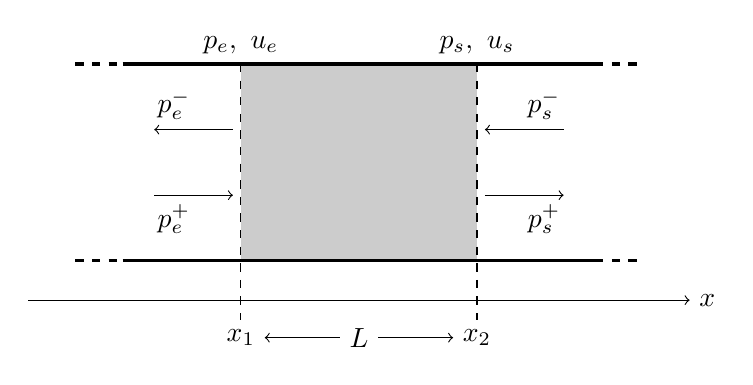
\begin{tikzpicture}
    \def\height{2.5};
    \def\length{6};
    \def\xone{\length/4};
    \def\xtwo{3*\length/4};
    \def\arrow{1};
    \def\xdist{9cm};
    
    \fill[black!20] (\xone,\height) rectangle (\xtwo,0);
    \draw[dashed] (\xone,\height) node[above] {$p_e,~u_e$} -- ++(0,-1.3*\height) node (x1) [below]{$x_1$};
    \draw[dashed] (\xtwo,\height) node[above]{$p_s,~u_s$} -- ++(0,-1.3*\height)node (x2) [below]{$x_2$};
    
    \draw[very thick,dashed] (-.1*\length,0) -- ++(.1*\length,0) coordinate(a1);
    \draw[very thick] (a1) -- ++(\length,0) coordinate(b1);
    \draw[very thick,dashed] (b1) -- ++(.1*\length,0);    
    \draw[very thick,dashed] (-.1*\length,\height) -- ++(.1*\length,0) coordinate(a2);
    \draw[very thick] (a2) -- ++(\length,0) coordinate(b2);
    \draw[very thick,dashed] (b2) -- ++(.1*\length,0);  
    
%    \draw[<-] (\xone-.1,\height/2) -- ++(-\arrow,0) node[midway]{\shortstack{$p_e$\\$u_e$}};
%    \draw[->] (\xtwo+.1,\height/2) -- ++(+\arrow,0) node[midway]{\shortstack{$p_s$\\$u_s$}};

	\draw[<-] (\xone-.1,\height/3) -- ++(-\arrow,0) node[near end, below]{$p_e^+$};
    \draw[->] (\xtwo+.1,\height/3) -- ++(+\arrow,0) node[near end, below]{$p_s^+$};
    \draw[->] (\xone-.1,2*\height/3) -- ++(-\arrow,0) node[near end, above]{$p_e^-$};
    \draw[<-] (\xtwo+.1,2*\height/3) -- ++(+\arrow,0) node[near end, above]{$p_s^-$};
    
    \draw[->] (-.2*\length,-.2*\height) --   ++(1.4*\length,0) node[right]{$x$};
    
    \draw[<->] (x1.east) -- (x2.west) node[midway, fill=white] {$L$};
    
%    \draw (a2) node[above]{\bf (a)};
    
    %%%%%
%    \begin{scope}[xshift=\xdist]
%    \fill[black!20] (\xone,\height) rectangle (\xtwo,0);
%    \draw[dashed] (\xone,\height) -- ++(0,-1.3*\height) node[below]{$x_1$};
%    \draw[dashed] (\xtwo,\height) -- ++(0,-1.3*\height)node[below]{$x_2$};
%    
%    \draw[very thick,dashed] (-.1*\length,0) -- ++(.1*\length,0) coordinate(a1);
%    \draw[very thick] (a1) -- ++(\length,0) coordinate(b1);
%    \draw[very thick,dashed] (b1) -- ++(.1*\length,0);    
%    \draw[very thick,dashed] (-.1*\length,\height) -- ++(.1*\length,0) coordinate(a2);
%    \draw[very thick] (a2) -- ++(\length,0) coordinate(b2);
%    \draw[very thick,dashed] (b2) -- ++(.1*\length,0);  
%    
%    \draw[->] (\xone-.1,\height/3) -- ++(-\arrow,0) node[midway,below]{$p_1^-$};
%    \draw[<-] (\xone-.1,2*\height/3) -- ++(-\arrow,0) node[midway,above]{$p_1^+$};
%    \draw[<-] (\xtwo+.1,\height/3) -- ++(+\arrow,0) node[midway,below]{$p_2^-$};
%    \draw[->] (\xtwo+.1,2*\height/3) -- ++(+\arrow,0) node[midway,above]{$p_2^+$};
%    
%    \draw[->] (-.2*\length,-.2*\height) --   ++(1.4*\length,0) node[above]{$x$};
%    
%    \draw (a2) node[above]{\bf (b)};
%    
%    \end{scope}
\end{tikzpicture}
    \caption{Représentations des ondes allers et retours dans une portion de tube.}%. \textbf{(a)} transfert, \textbf{(b)} diffusion.}
    \label{fig:WavesInDuctPiece}
\end{figure}



%Si l'on s'intéresse à un domaine à l'intérieur du tube telle que la zone grisée sur la figure~\ref{fig:WavesInDuctPiece} (une portion de tube, un stack, etc.), il peut être judicieux d'exprimer les ondes qui sortent de ce domaine en fonction de celles qui y entrent. La relation obtenue peut se mettre sous la forme d'une matrice de diffusion qui s'écrit
%
%\begin{equation}
%    \begin{pmatrix}
%        p_2^+\\
%        p_1^-
%    \end{pmatrix}=\begin{bmatrix}
%        \mathcal T^+ & \mathcal R^-\\
%        \mathcal R^+ & \mathcal T^-
%    \end{bmatrix}\begin{pmatrix}
%        p_1^+\\
%        p_2^-
%    \end{pmatrix},
%    \label{eq:SMatrixRT}
%\end{equation}
%où $p_1^-$ et $p_2^+$ sont les ondes de pression sortantes du domaine, et $p_1^+$ et $p_2^-$ sont les ondes entrantes. Les coefficients de la matrice de diffusion sont définis par
%
%\begin{subequations}
%    \begin{align}
%        \mathcal T^+ &= \frac{2(T_{pp}T_{uu}-T_{pu}T_{up})}{T_{pp}+T_{uu}-(T_{pu}/Z_c+T_{up}Z_c)},\label{eq:SMatrixT+}\\\vspace{1em}
%        \mathcal R^- &= \frac{T_{up}Z_c-T_{pu}/Z_c+T_{pp}-T_{uu}}{T_{pp}+T_{uu}-(T_{pu}/Z_c+T_{up}Z_c)},\label{eq:SMatrixR-}\\\vspace{.5em}
%        \mathcal R^+ &= \frac{T_{up}Z_c-T_{pu}/Z_c-T_{pp}+T_{uu}}{T_{pp}+T_{uu}-(T_{pu}/Z_c+T_{up}Z_c)}, \text{et}\label{eq:SMatrixR+}\\
%        \mathcal T^- &= \frac{2}{T_{pp}+T_{uu}-(T_{pu}/Z_c+T_{up}Z_c)}.\label{eq:SMatrixT-}
%    \end{align}
%    \label{eq:SMatrixCoeff}%
%\end{subequations}

\subsubsection{Matrice de transfert d'un noyau thermoacoustique}

Comme déjà expliqué plus haut, le processus thermoacoustique se produit dans un matériau poreux placé dans le guide d'ondes des machines thermoacoustiques. La définition des termes constituant la matrice de transfert change alors légèremement pour prendre en compte sa porosité $\Phi$ selon l'équation

\begin{equation}
\begin{pmatrix}
p_s\\
u_s
\end{pmatrix} = \begin{bmatrix}
\cos(k_x L) & -i\frac{\rho_0 c_0}{\Phi S}\sin(k_x L)\\
-i\frac{\Phi S}{\rho_0 c_0}\sin(k_x L) & \cos(k_x L)
\end{bmatrix}
\begin{pmatrix}
p_e\\
u_e
\end{pmatrix}.\label{eq:Tmatrix_poreux}
\end{equation}


La représentation du circuit sur la figure~\ref{fig:CircEquivTAC} se traduit au moyen de matrice de transfert à l'ordre 1 par 


\begin{equation}
	\begin{pmatrix}
		p + \deriv p\\
		u + \deriv u
	\end{pmatrix} = \begin{bmatrix}
	1 & -\left(i\omega L + R_\nu\right)~\deriv x  \\
	-\left(\frac{1}{R_\kappa} + i \omega C\right)~\deriv x & g~\deriv x \end{bmatrix} \begin{pmatrix}
	p \\
	u
	\end{pmatrix}, \label{eq:TMatrix_NoyauTA}
\end{equation}
ou bien même en simplifiant encore plus les choses par

\begin{equation}
    \begin{pmatrix}
        p + \deriv p \\
        u + \deriv u
    \end{pmatrix} = \begin{bmatrix}
    1 & -R_\nu \\
    0 & 1
    \end{bmatrix}\begin{pmatrix}
        p \\
        u
    \end{pmatrix}.
    \label{eq:Tmatrix_NoyauTA_simplifie}
\end{equation}


Enfin, si le matériau poreux est long, il est possible de le représenter par une succession de $N$ portions élémentaires du poreux et donc un produit de matrices de transfert

\begin{equation}
\begin{pmatrix}
p_s\\
u_s
\end{pmatrix} = \prod_{n=0}^{N-1} \begin{bmatrix}
T_{pp}^{(n)} & T_{pu}^{(n)}\\
T_{up}^{(n)} & T_{uu}^{(n)}
\end{bmatrix}\begin{pmatrix}
p_e\\
u_e
\end{pmatrix}.
\label{eq:TMatrix_prod_TppTuu}
\end{equation}

\section{Limites des modèles}

%\begin{itemize}
%    \item Streaming
%    \item Convection naturelle
%    \item Hypothèse 1D invalide
%    \item Génération d'harmoniques par les sources ? vérifier si superposition d'effet à 47 Hz avec 2x47 Hz etc.
%\end{itemize}

Bien que la théorie linéaire de Rott, au travers notamment de logiciels de simulations spécialisés tels que \textsc{DeltaEC}, soit suffisante pour prédire le comportement des machines thermoacoustiques de même que leurs performances, de nombreux effets sont négligés~\cite{DeltaEC}. Le vent acoustique \cite{so_internal_2006, bailliet_acoustic_2001, ramadan_experimental_2018}, les écoulements turbulents et la formations de tourbillons, la génération d'harmoniques supérieures et la convection naturelle sont autant d'effets non linéaires qui ne respectent pas les hypothèses retenues pour les modèles. Ce dernier effet est assez peu étudié, bien qu'il a déjà été observé que le déclenchement de moteurs thermoacoustique y est très sensible et que les températures le long des dimensions transverses du noyau peuvent être inhomogènes \cite{ross_influence_2003, ramadan_experimental_2018, hireche_numerical_2019}. Dans le cas des pompes à chaleur et réfrigérateurs pour lesquelles les gradients de températures sont plus faible que pour les moteurs, la littérature sur la convection naturelle est encore plus rare, ce qui motive ce projet de recherche \cite{zhang_novel_2011, babaei_investigation_2010}.\echaf{à suivre}

\section{Plan du manuscrit}
Après avoir présenté les éléments de base du travail sur ce réfrigérateur thermoacoustique \textsc{Tacot}, le contexte autour de cette thèse, et l'axe sur lequel elle se concentre, un plan est proposé.\medskip

Dans le chapitre~\ref{chap:DispositifExpe}, le  \nameref{chap:DispositifExpe} est présenté. Cela inclut une présentation de la géométrie du refrigérateur, l'instrumentation utilisée pour les acquisitions, le déroulé d'une expérience, et les conditions de chacune d'entre elle. L'accent est porté sur l'étude de la convection naturelle, et les orientations du réfrigérateur choisies pour répondre aux hypothèses auxquelles il faut apporter des réponses sont définies.\smallskip

Le chapitre~\ref{chap:SimusRealisees} introduit les \nameref{chap:SimusRealisees} dans le but de comprendre le fonctionnement du réfrigérateur au-delà de ce que prédit la théorie linéaire en prenant en compte plus de phénomènes. La première simulation est  plus un prétexte à l'introduction des quantité adimensionnelles couramment utilisées en mécanique des fluides. En particulier, l'étude du nombre de Rayleigh permet d'anticiper la présence ou l'absence d'un courant de convection naturelle dans différentes zones du réfrigérateur. Suite à cela, un modèle numérique du régime stationnaire par éléments finis et réalisé avec le logiciel \textsc{Comsol} Multiphysics\textss\textregistered est présenté. Ce modèle, pour rester simple tout en représentant plus de phénomènes, simule le comportement purement thermique d'un système équivalent. Enfin, un modèle analytique du régime transitoire est proposé, en prenant en compte les mêmes phénomènes que dans la simulation numérique.\smallskip

Le chapitre~\ref{chap:EtudeExpe} est dédié aux \nameref{chap:EtudeExpe}. \smallskip

Chap~\ref{chap:Conc} - \nameref{chap:Conc}.\smallskip

\ref{chap:Persp} - \nameref{chap:Persp}.


